%  LaTeX support: latex@mdpi.com 
%  In case you need support, please attach all files that are necessary for compiling as well as the log file, and specify the details of your LaTeX setup (which operating system and LaTeX version / tools you are using).

%=================================================================
\documentclass[journal,article,submit,moreauthors,pdftex]{Definitions/mdpi} 

% If you would like to post an early version of this manuscript as a preprint, you may use preprint as the journal and change 'submit' to 'accept'. The document class line would be, e.g., \documentclass[preprints,article,accept,moreauthors,pdftex]{mdpi}. This is especially recommended for submission to arXiv, where line numbers should be removed before posting. For preprints.org, the editorial staff will make this change immediately prior to posting.

%--------------------
% Class Options:
%--------------------
%----------
% journal
%----------
% Choose between the following MDPI journals:
% biologics, jmp, eng, jor, nursrep, biophysica, gastroent, jox, adolescents, hygiene, taxonomy, business, nanomanufacturing, geography, compoundsacoustics, actuators, addictions, admsci, aerospace, agriculture, agriengineering, agronomy, ai, algorithms, allergies, analytica, animals, antibiotics, antibodies, antioxidants, applmech, applnano, applsci, arts, asc, asi, atmosphere, atoms, automation, axioms, batteries, bdcc, behavsci , beverages, bioengineering, biology, biomedicines, biomedinformatics, biomimetics, biomolecules, biosensors, bloods, brainsci, breath, buildings, cancers, carbon , catalysts, cells, ceramics, challenges, chemengineering, chemistry, chemosensors, chemproc, children, civileng, cleantechnol, climate, clockssleep, cmd, coatings, colloids, computation, computers, condensedmatter, cosmetics, cryptography, crystals, cyber, dairy, data, dentistry, dermatopathology, designs, diabetology, diagnostics, digital, diseases, diversity, drones, earth, econometrics, ecologies, economies, education, ejbc, ejihpe, electricity, electrochem, electronicmat, electronics, endocrines, energies, engproc, entropy, environments, environsciproc, epidemiologia, epigenomes, est, fermentation, fibers, fire, fishes, fluids, foods, forecasting, forests, fractalfract, fuels, futureinternet, futurephys, galaxies, games, gardens, gases, gastrointestdisord, gels, genealogy, genes, geohazards, geosciences, geriatrics, hazardousmatters, healthcare, hearts, heritage, highthroughput, horticulturae, humanities, hydrogen, hydrology, ijerph, ijfs, ijgi, ijms, ijtpp, immuno, informatics, information, infrastructures, inorganics, insects, instruments, inventions, iot, j, jcdd, jce, jcm, jcp, jcs, jdb, jfb, jfmk, jimaging, jintelligence, jlpea, jmmp, jmse, jne, jnt, jof, joitmc, journalmedia, jpm, jrfm, jsan, land, languages, laws, life, literature, livers, logistics, lubricants, machines, magnetochemistry, make, marinedrugs, materials, materproc, mathematics, mca, medicina, medicines, medsci, membranes, metabolites, metals, microarrays, micromachines, microorganisms, minerals, modelling, molbank, molecules, mps, mti, nanomaterials, ncrna, ijns, neurosci, neuroglia, nitrogen, notspecified, nutrients, obesities, oceans, ohbm, osteology, optics, organics, particles, pathogens, pharmaceuticals, pharmaceutics, pharmacy, philosophies, photonics, physics, plants, plasma, pollutants, polymers, polysaccharides, preprints , proceedings, processes, prosthesis, proteomes, psych, psychiatryint, publications, quantumrep, quaternary, qubs, radiation, reactions, recycling, religions, remotesensing, reprodmed, reports, resources, risks, robotics, safety, sci, scipharm, sensors, separations, sexes, signals, sinusitis, skins, smartcities, sna, societies, socsci, soilsystems, solids, sports, standards, stats, surfaces, surgeries, suschem, sustainability, world, symmetry, systems, technologies, telecom, test, tourismhosp, toxics, toxins, transplantology, tropicalmed, universe, urbansci, uro, vaccines, vehicles, vetsci, vibration, viruses, vision, water, wem, wevj, women

%---------
% article
%---------
% The default type of manuscript is "article", but can be replaced by: 
% abstract, addendum, article, benchmark, book, bookreview, briefreport, casereport, changes, comment, commentary, communication, conceptpaper, conferenceproceedings, correction, conferencereport, expressionofconcern, extendedabstract, meetingreport, creative, datadescriptor, discussion, editorial, essay, erratum, hypothesis, interestingimages, letter, meetingreport, newbookreceived, obituary, opinion, projectreport, reply, retraction, review, perspective, protocol, shortnote, supfile, technicalnote, viewpoint
% supfile = supplementary materials

%----------
% submit
%----------
% The class option "submit" will be changed to "accept" by the Editorial Office when the paper is accepted. This will only make changes to the frontpage (e.g., the logo of the journal will get visible), the headings, and the copyright information. Also, line numbering will be removed. Journal info and pagination for accepted papers will also be assigned by the Editorial Office.

%------------------
% moreauthors
%------------------
% If there is only one author the class option oneauthor should be used. Otherwise use the class option moreauthors.

%---------
% pdftex
%---------
% The option pdftex is for use with pdfLaTeX. If eps figures are used, remove the option pdftex and use LaTeX and dvi2pdf.

%=================================================================
\firstpage{1} 
\makeatletter 
\setcounter{page}{\@firstpage} 
\makeatother
\pubvolume{xx}
\issuenum{1}
\articlenumber{5}
\pubyear{2020}
\copyrightyear{2020}
%\externaleditor{Academic Editor: name}
\history{Received: date; Accepted: date; Published: date}
%\updates{yes} % If there is an update available, un-comment this line

%% MDPI internal command: uncomment if new journal that already uses continuous page numbers 
%\continuouspages{yes}

%------------------------------------------------------------------
% The following line should be uncommented if the LaTeX file is uploaded to arXiv.org
%\pdfoutput=1

%=================================================================
% Add packages and commands here. The following packages are loaded in our class file: fontenc, inputenc, calc, indentfirst, fancyhdr, graphicx,epstopdf, lastpage, ifthen, lineno, float, amsmath, setspace, enumitem, mathpazo, booktabs, titlesec, etoolbox, tabto, xcolor, soul, multirow, microtype, tikz, totcount, amsthm, hyphenat, natbib, hyperref, footmisc, url, geometry, newfloat, caption

%=================================================================
%% Please use the following mathematics environments: Theorem, Lemma, Corollary, Proposition, Characterization, Property, Problem, Example, ExamplesandDefinitions, Hypothesis, Remark, Definition, Notation, Assumption
%% For proofs, please use the proof environment (the amsthm package is loaded by the MDPI class).

%=================================================================
% Full title of the paper (Capitalized)
\Title{Title}

% Author Orchid ID: enter ID or remove command
\newcommand{\orcidauthorA}{0000-0000-000-000X} % Add \orcidA{} behind the author's name
%\newcommand{\orcidauthorB}{0000-0000-000-000X} % Add \orcidB{} behind the author's name

% Authors, for the paper (add full first names)
\Author{Firstname Lastname $^{1,\dagger,\ddagger}$\orcidA{}, Firstname Lastname $^{1,\ddagger}$ and Firstname Lastname $^{2,}$*}


% Authors, for metadata in PDF
\AuthorNames{Firstname Lastname, Firstname Lastname and Firstname Lastname}

% Affiliations / Addresses (Add [1] after \address if there is only one affiliation.)
\address{%
$^{1}$ \quad Affiliation 1; e-mail@e-mail.com\\
$^{2}$ \quad Affiliation 2; e-mail@e-mail.com}

% Contact information of the corresponding author
\corres{Correspondence: e-mail@e-mail.com; Tel.: (optional; include country code; if there are multiple corresponding authors, add author initials) +xx-xxxx-xxx-xxxx (F.L.)}

% Current address and/or shared authorship
\firstnote{Current address: Affiliation 3} 
\secondnote{These authors contributed equally to this work.}
% The commands \thirdnote{} till \eighthnote{} are available for further notes

%\simplesumm{} % Simple summary

%\conference{} % An extended version of a conference paper

% Abstract (Do not insert blank lines, i.e. \\) 
\abstract{A single paragraph of about 200 words maximum. For research articles, abstracts should give a pertinent overview of the work. We strongly encourage authors to use the following style of structured abstracts, but without headings: (1) Background: Place the question addressed in a broad context and highlight the purpose of the study; (2) Methods: Describe briefly the main methods or treatments applied; (3) Results: Summarize the article's main findings; and (4) Conclusion: Indicate the main conclusions or interpretations. The abstract should be an objective representation of the article, it must not contain results which are not presented and substantiated in the main text and should not exaggerate the main conclusions.}

% Keywords
\keyword{keyword 1; keyword 2; keyword 3}  % List three to ten pertinent keywords specific to the article, yet reasonably common within the subject discipline.

% The fields PACS, MSC, and JEL may be left empty or commented out if not applicable
%\PACS{J0101}
%\MSC{}
%\JEL{}

%%%%%%%%%%%%%%%%%%%%%%%%%%%%%%%%%%%%%%%%%%
% Only for the journal Diversity
%\LSID{\url{http://}}

%%%%%%%%%%%%%%%%%%%%%%%%%%%%%%%%%%%%%%%%%%
% Only for the journal Applied Sciences:
%\featuredapplication{Authors are encouraged to provide a concise description of the specific application or a potential application of the work. This section is not mandatory.}
%%%%%%%%%%%%%%%%%%%%%%%%%%%%%%%%%%%%%%%%%%

%%%%%%%%%%%%%%%%%%%%%%%%%%%%%%%%%%%%%%%%%%
% Only for the journal Data:
%\dataset{DOI number or link to the deposited data set in cases where the data set is published or set to be published separately. If the data set is submitted and will be published as a supplement to this paper in the journal Data, this field will be filled by the editors of the journal. In this case, please make sure to submit the data set as a supplement when entering your manuscript into our manuscript editorial system.}

%\datasetlicense{license under which the data set is made available (CC0, CC-BY, CC-BY-SA, CC-BY-NC, etc.)}

%%%%%%%%%%%%%%%%%%%%%%%%%%%%%%%%%%%%%%%%%%
% Only for the journal Toxins
%\keycontribution{The breakthroughs or highlights of the manuscript. Authors can write one or two sentences to describe the most important part of the paper.}

%\setcounter{secnumdepth}{4}
%%%%%%%%%%%%%%%%%%%%%%%%%%%%%%%%%%%%%%%%%%
\begin{document}
%%%%%%%%%%%%%%%%%%%%%%%%%%%%%%%%%%%%%%%%%%
\section{Introduction}
The introduction should briefly place the study in a broad context and highlight why it is important. It should define the purpose of the work and its significance. The current state of the research field should be reviewed carefully and key publications cited. Please highlight controversial and diverging hypotheses when necessary. Finally, briefly mention the main aim of the work and highlight the principal conclusions. As far as possible, please keep the introduction comprehensible to scientists outside your particular field of research. Citing a journal paper \cite{ref-journal}. And now citing a book reference \cite{ref-book}. Please use the command \citep{ref-journal} for the following MDPI journals, which use author-date citation: Administrative Sciences, Arts, Econometrics, Economies, Genealogy, Humanities, IJFS, JRFM, Languages, Laws, Religions, Risks, Social Sciences.
\section{Main result}
In airlines, the spatial distribution of aircraft stations is a non-Euclidean structure, that is, the number of stations around each station is uncertain, and even if two stations are adjacent, they may not actually communicate with each other, resulting in no spatial relationship between their traffic. Therefore, traditional convolutional neural network (CNN) cannot accurately obtain their spatial information. At this point, multiple sites can be abstracted into A graph (see Figure \ref{fig:stations}). Features are extracted from the original input data to obtain the result of feature mapping of multiple channels. The intercommunication relationship between each site is represented by adjacency matrix A.
\begin{figure}[htp]
    \centering
    % \includegraphics[width=8 cm]{Definitions/logo/-mdpi}
    \caption{The distribution of the stations.}
    \label{fig:stations}
\end{figure}
\subsection{The definition of the problem } 
The problem of airline passenger flow prediction can be described as follows: the historical flow data of each station $X_{t-s}, X_{t-s+1},  X_{t-2}, \cdots,  X_{t-1}$ (s is the time step) can be used to predict the flow $X_{t}$ of the next period. 
The formula is described as
\begin{equation}
    X_{t} = F([ X_{t-s}, X_{t-s+1}, \cdots, X_{t-2}, X_{t-1}])
\end{equation}
where, $X$ is the site characteristics at each time step, and $F$ is a nonlinear function.
\par In the actual traffic system, the road network is regarded as A directed graph $G = (q, V, A)$. Each sensor in the road network is regarded as a node vi V and its value Q R is a scalar. V RN and N is the number of sensors. 
The flow relationship between nodes consists of adjacency matrix A that is, the element Aij in A represents the connection relationship between node VI and vJ.
\subsection{The description of the GCN} 
When dealing with the structure of the graph, it is necessary to obtain its Laplace matrix L first, which is generally defined in the following ways:
\begin{equation}
    L=D^{-\frac{1}{2}}(D-A) D^{-\frac{1}{2}}=I_{N}-D^{-\frac{1}{2}} A D^{-\frac{1}{2}}
\end{equation}
Where, $I_{N}$is the identity matrix of $N×N$; Degree matrix $D$ is defined as $D_{i i}=\sum_{i} A_{i j}^{i}$. Decompose the eigenvalue of $L$ to get $L = \mathrm{L}=\mathrm{U} \Lambda \mathrm{U}^{\mathrm{T}}$. $\Lambda$ is made up of L eigenvalues of diagonal matrix. $\mathrm{U}=\left\{\mathrm{u}_{1}, \mathrm{u}_{2}, \ldots, \mathrm{u}_{\mathrm{N}}\right\}$ is composed of the eigenvector L, and it is an orthonormal basis for $\mathrm{R}^{\mathrm{N}}$.
\par The spectral convolution theory in the graph structure has been supplemented and perfected in the paper. The convolution operation of convolution kernel $G$ and input signal $X$ in the time domain can be converted into the inner product form in the frequency domain.
\begin{equation}
    \left.g^{*} x=U\left(U^{\mathrm{T}} g\right) \odot\left(U^{\mathrm{T}} \boldsymbol{x}\right)\right)=U_{g_{\theta}}(A) U^{\mathrm{T}} x
\end{equation}
where $g_{s}(\Lambda)=U^{T} g=\operatorname{diag}(\theta), \theta \in R^{N}$, $\odot$ represents the hadamar product, $U^{T}g$means mapping $g$ to the frequency domain space based on $U$. Due to $g_{\theta}$ high computational complexity, so using hierarchical linear model constraints and the chebyshev polynomial to approximate calculation. In this paper, The simplified first order polynomial form of $g*x$ is adopted.
\begin{equation}
    g^{*} x=U_{g_{\theta}} U_{x}^{\mathrm{T}} \approx \theta\left(I_{N}+D^{-1 / 2} A D^{-1 / 2}\right) x
\end{equation}
where $\widetilde{D}^{-1 / 2} \widetilde{A} \widetilde{D}^{-1 / 2}=I_{N}+D^{-1 / 2} A D^{-1 / 2} \quad \tilde{A}=I_{N}+A $, ${D}=\sum_{i} \widetilde{A}_{i j}$, Therefore, the output of layer $L$ is
\begin{equation}
    H^{(l)}=\sigma\left(\widetilde{D}^{-\frac{1}{2}} \widetilde{A} \widetilde{D}^{-\frac{1}{2}} H^{(l-1)} W^{(l)}\right.
\end{equation}
where $\delta$ is the activation function, $\widetilde{W}^{(l)}=\theta^{(l-1)} W^{(l)} \quad \boldsymbol{\theta}^{(l-1)} \in \boldsymbol{R}^{c^{(1-l)} \times F^{(l-1)}}, \boldsymbol{W}^{(l)} \in \boldsymbol{R}^{F^{(l-1)} \times c^{(l)}}$,  $C^{(L-1)}$ is the output dimension of the $(L-1)$ layer, and $F^{(L-1)}$ is the characteristic vector size of each dimension. Therefore
\begin{equation}
    H^{(l)}=\sigma\left(\widetilde{D}^{-\frac{1}{2}} \widetilde{A} \widetilde{D}^{-\frac{1}{2}} H^{(l-1)} \widetilde{W}^{(l)}\right)
\end{equation}
\par At present, there is no effective measurement method for the calculation of adjacency matrix $A$. Most scholars use heuristic methods, that is, based on the Euclidean distance or Markov distance between sensors to determine the element value corresponding to the adjacency matrix. However, these methods all require manual calculation of the distance relationship between the sensors in advance. In this paper, the data-driven method is adopted to calculate the adjacency matrix, and $A = D$, then the formula can be written as:
\begin{equation}
    \left.H^{(l)}=\sigma / \widetilde{A} H^{(l-1)} \widetilde{W}^{(l)}\right)
    \label{equ:hl}
\end{equation}
The element value of matrix $A$ is learned from the sample data, that is, the matrix is composed of trainable parameters. The data-driven approach is more realistic than the heuristic approach. Therefore, the L layer of the convolutional neural network is constructed in accordance with Formula \ref{equ:hl}. It should be noted that the initial $A$ maki is the same for each layer of the convolutional network, and the parameters are updated only when the error is propagated backwards.
\subsection{the import of LSTM}
It is found that Recurrent Neural networks (RNN) are widely used in sequential data such as natural language and image processing, which have a significant effect. Since then, various types of circulating neural networks have been proposed. Aiming at the problem of air passenger flow prediction, this paper introduces the long and short term memory network, which can extract the characteristic information of the input sequence and find its internal relation, so as to improve the prediction accuracy of the model.
\par The LSTM network structure used in this paper is shown as follows
\begin{figure}
    \centering
    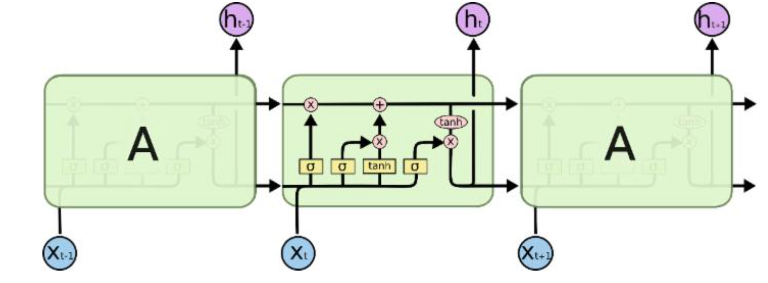
\includegraphics[width=8 cm]{./imgs/LSTMpng.png}
    \caption{The structure of LSTM.}
\end{figure}
The network model mainly accepts three inputs: $X$, $H$ and $C$ represent the current state, hidden layer state and cell state, respectively.
\par LSTM mainly realizes the management of long and short term memory through three gating units. The first step in the LSTM is to determine what information needs to be thrown out of the cell state. This decision is made by a sigmoID layer called the "Forget Gate." Input x and h, output a number between 0 and 1. 1 means "keep the value completely", while 0 means "throw the value away completely". The formula of forgetting gate is as follows:
\begin{equation}
    f_{t}=\sigma\left(W_{f} \cdot\left[h_{t-1}, x_{t}\right]+b_{f}\right)
\end{equation}
where $W_{f}$ and $b_{f}$ are the parameters to be learned, and $\sigma$ is the sigmod activation function.
\par The second step is to determine what information we need to store in the Cell State. There are two parts to this question. First, a sigmod layer calls the "Input Gate" to determine which data needs to be updated. Then, a tanh layer creates a vector C1 for the new candidate values, which can be added to the state.
\begin{equation}
    \begin{aligned}
    i_{t} &=\sigma\left(W_{i} \cdot\left[h_{t-1}, x_{t}\right]+b_{i}\right) \\
    \tilde{C}_{t} &=\tanh \left(W_{C} \cdot\left[h_{t-1}, x_{t}\right]+b_{C}\right)
    \end{aligned}
\end{equation}
\par After deciding what needs to be forgotten and what needs to be added, the old cell state Ct-1 can be updated to the new cell state Ct.
\begin{equation}
    C_{t}=f_{t} * C_{t-1}+i_{t} * \tilde{C}_{t}
\end{equation}
\par Finally, we need to decide what to export. This output is based on our cell state, but will be a filtered part of the value. First, we run an output gate to determine which part of the cell state we are going to output. Then we put the cell state into the tanh (pressing the value between -1 and 1), and finally we multiply it by the output of the output gate.
\begin{equation}
    \begin{array}{l}
    o_{t}=\sigma\left(W_{o}\left[h_{t-1}, x_{t}\right]+b_{o}\right) \\
    h_{t}=o_{t} * \tanh \left(C_{t}\right)
    \end{array}
\end{equation}
\subsection{The description of algorithm}
The network structure based on GCN-LSTM model proposed in this paper is shown in the figure. The prediction model is composed of multiple layers of GCN and an LSTM model. Among them, GCN model is mainly used to extract the features of graph networks, while LSTM network model is mainly used to solve the long-term and short-term dependence between data. 
\par In this paper, features of different graph networks are extracted through multiple GCN, and the extracted features are transferred into LSTM, and the timing characteristics of sequence data are analyzed through LSTM, and a more accurate prediction value is given through multi-layer full connection layer.
\begin{figure}[htp]
    \centering
    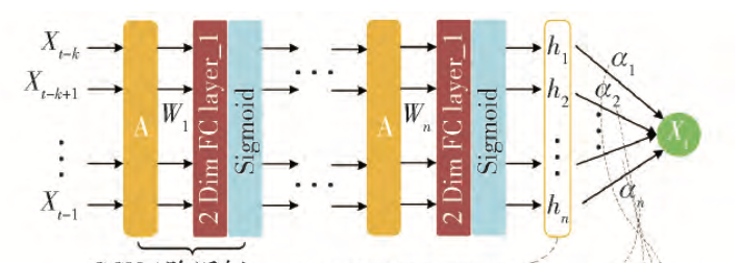
\includegraphics[width=8 cm]{./imgs/GCN-LSTM.png}
    \caption{Overall structure of GCN-LSTM model (original features of air passenger flow data are extracted by using first-order approximate GCN, and output features are analyzed by LSTM for long-term and short-term sequence characteristics, and then predicted values are obtained).}
\end{figure}
%%%%%%%%%%%%%%%%%%%%%%%%%%%%%%%%%%%%%%%%%%
\section{Patents}
This section is not mandatory, but may be added if there are patents resulting from the work reported in this manuscript.

%%%%%%%%%%%%%%%%%%%%%%%%%%%%%%%%%%%%%%%%%%
\vspace{6pt} 

%%%%%%%%%%%%%%%%%%%%%%%%%%%%%%%%%%%%%%%%%%
%% optional
%\supplementary{The following are available online at \linksupplementary{s1}, Figure S1: title, Table S1: title, Video S1: title.}

% Only for the journal Methods and Protocols:
% If you wish to submit a video article, please do so with any other supplementary material.
% \supplementary{The following are available at \linksupplementary{s1}, Figure S1: title, Table S1: title, Video S1: title. A supporting video article is available at doi: link.}

%%%%%%%%%%%%%%%%%%%%%%%%%%%%%%%%%%%%%%%%%%
\authorcontributions{For research articles with several authors, a short paragraph specifying their individual contributions must be provided. The following statements should be used ``Conceptualization, X.X. and Y.Y.; methodology, X.X.; software, X.X.; validation, X.X., Y.Y. and Z.Z.; formal analysis, X.X.; investigation, X.X.; resources, X.X.; data curation, X.X.; writing--original draft preparation, X.X.; writing--review and editing, X.X.; visualization, X.X.; supervision, X.X.; project administration, X.X.; funding acquisition, Y.Y. All authors have read and agreed to the published version of the manuscript.'', please turn to the  \href{http://img.mdpi.org/data/contributor-role-instruction.pdf}{CRediT taxonomy} for the term explanation. Authorship must be limited to those who have contributed substantially to the work reported.}

%%%%%%%%%%%%%%%%%%%%%%%%%%%%%%%%%%%%%%%%%%
\funding{Please add: ``This research received no external funding'' or ``This research was funded by NAME OF FUNDER grant number XXX.'' and  and ``The APC was funded by XXX''. Check carefully that the details given are accurate and use the standard spelling of funding agency names at \url{https://search.crossref.org/funding}, any errors may affect your future funding.}

%%%%%%%%%%%%%%%%%%%%%%%%%%%%%%%%%%%%%%%%%%
\acknowledgments{In this section you can acknowledge any support given which is not covered by the author contribution or funding sections. This may include administrative and technical support, or donations in kind (e.g., materials used for experiments).}

%%%%%%%%%%%%%%%%%%%%%%%%%%%%%%%%%%%%%%%%%%
\conflictsofinterest{Declare conflicts of interest or state ``The authors declare no conflict of interest.'' Authors must identify and declare any personal circumstances or interest that may be perceived as inappropriately influencing the representation or interpretation of reported research results. Any role of the funders in the design of the study; in the collection, analyses or interpretation of data; in the writing of the manuscript, or in the decision to publish the results must be declared in this section. If there is no role, please state ``The funders had no role in the design of the study; in the collection, analyses, or interpretation of data; in the writing of the manuscript, or in the decision to publish the results''.} 

%%%%%%%%%%%%%%%%%%%%%%%%%%%%%%%%%%%%%%%%%%
%% optional
\abbreviations{The following abbreviations are used in this manuscript:\\

\noindent 
\begin{tabular}{@{}ll}
MDPI & Multidisciplinary Digital Publishing Institute\\
DOAJ & Directory of open access journals\\
TLA & Three letter acronym\\
LD & linear dichroism
\end{tabular}}

%%%%%%%%%%%%%%%%%%%%%%%%%%%%%%%%%%%%%%%%%%
%% optional
\appendixtitles{no} % Leave argument "no" if all appendix headings stay EMPTY (then no dot is printed after "Appendix A"). If the appendix sections contain a heading then change the argument to "yes".
\appendix
\section{}
\unskip
\subsection{}
The appendix is an optional section that can contain details and data supplemental to the main text. For example, explanations of experimental details that would disrupt the flow of the main text, but nonetheless remain crucial to understanding and reproducing the research shown; figures of replicates for experiments of which representative data is shown in the main text can be added here if brief, or as Supplementary data. Mathematical proofs of results not central to the paper can be added as an appendix.

\section{}
All appendix sections must be cited in the main text. In the appendixes, Figures, Tables, etc. should be labeled starting with `A', e.g., Figure A1, Figure A2, etc. 

%%%%%%%%%%%%%%%%%%%%%%%%%%%%%%%%%%%%%%%%%%
\reftitle{References}

% Please provide either the correct journal abbreviation (e.g. according to the “List of Title Word Abbreviations” http://www.issn.org/services/online-services/access-to-the-ltwa/) or the full name of the journal.
% Citations and References in Supplementary files are permitted provided that they also appear in the reference list here. 

%=====================================
% References, variant A: external bibliography
%=====================================
\externalbibliography{yes}
\bibliography{mybib}

%=====================================
% References, variant B: internal bibliography
%=====================================
% \begin{thebibliography}{999}
% % Reference 1
% \bibitem[Author1(year)]{ref-journal}
% Author1, T. The title of the cited article. {\em Journal Abbreviation} {\bf 2008}, {\em 10}, 142--149.
% % Reference 2
% \bibitem[Author2(year)]{ref-book}
% Author2, L. The title of the cited contribution. In {\em The Book Title}; Editor1, F., Editor2, A., Eds.; Publishing House: City, Country, 2007; pp. 32--58.
% \end{thebibliography}

% The following MDPI journals use author-date citation: Arts, Econometrics, Economies, Genealogy, Humanities, IJFS, JRFM, Laws, Religions, Risks, Social Sciences. For those journals, please follow the formatting guidelines on http://www.mdpi.com/authors/references
% To cite two works by the same author: \citeauthor{ref-journal-1a} (\citeyear{ref-journal-1a}, \citeyear{ref-journal-1b}). This produces: Whittaker (1967, 1975)
% To cite two works by the same author with specific pages: \citeauthor{ref-journal-3a} (\citeyear{ref-journal-3a}, p. 328; \citeyear{ref-journal-3b}, p.475). This produces: Wong (1999, p. 328; 2000, p. 475)


%%%%%%%%%%%%%%%%%%%%%%%%%%%%%%%%%%%%%%%%%%
%% optional
\sampleavailability{Samples of the compounds ...... are available from the authors.}

%% for journal Sci
%\reviewreports{\\
%Reviewer 1 comments and authors’ response\\
%Reviewer 2 comments and authors’ response\\
%Reviewer 3 comments and authors’ response
%}

%%%%%%%%%%%%%%%%%%%%%%%%%%%%%%%%%%%%%%%%%%
\end{document}

